% Template for ICASSP-2015 paper; to be used with:
%          spconf.sty  - ICASSP/ICIP LaTeX style file, and
%          IEEEbib.bst - IEEE bibliography style file.
% --------------------------------------------------------------------------
\documentclass{article}
\usepackage{spconf,amsmath,graphicx,qtree,tabularx}
\usepackage{times}
\usepackage{latexsym}
\usepackage{graphicx}
\usepackage{listings}

\usepackage{tikz}
\usetikzlibrary{positioning}

% Example definitions.
% --------------------
\def\x{{\mathbf x}}
\def\L{{\cal L}}

% Title.
% ------
\title{AUDIO RENDERING OF MATHEMATICAL EQUATIONS}%
% Single address.
% ---------------
\name{Venkatesh Potluri, Saikrishna Rallabandi, Priyanka Srivastava, Kishore Prahallad}
\address{International Institute of Information Technology, Hyderabad}
%
% For example:
% ------------
%\address{School\\
%	Department\\
%	Address}
%
% Two addresses (uncomment and modify for two-address case).
% ----------------------------------------------------------
%\twoauthors
%  {A. Author-one, B. Author-two\sthanks{Thanks to XYZ agency for funding.}}
%	{School A-B\\
%	Department A-B\\
%	Address A-B}
%  {C. Author-three, D. Author-four\sthanks{The fourth author performed the work
%	while at ...}}
%	{School C-D\\
%	Department C-D\\
%	Address C-D}
%
\begin{document}
%\ninept
%
\maketitle
%
\begin{abstract}
Text to speech (TTS) systems hold promise as an information access tool for literate and illiterate including visually challenged. However, auditory rendering of mathematical content, specifically equation reading can not be effectively accomplished with the current systems.  Mathematical equations have to be read so that appropriate bracketing such as parentheses, superscripts and subscripts are unambiguously conveyed to the listener. Earlier works have attempted to use pauses as acoustic cues to indicate some of these. In this paper, we perform an experiment to measure the effectiveness of mathematical equations synthesised using a traditional TTS system. We analyse the acoustic cues which human-beings employ while speaking the mathematical content to (visually challenged) listeners and propose four techniques which render the observed patterns in a text-to- speech system. The evaluation considered eight aspects such as listening effort and intonation.We also performed a comprehension test by rendering mathematics using one of the proposed techniques on visually challenged people, who were able to solve the problems with 95\% accuracy with the proposed technique while a very meagre 30\% with the current state of the art technology. 
  
\end{abstract}
%
\begin{keywords}
Mathematical Equations, Multidimensional Audio, Paralinguistic cues, Text To speech
\end{keywords}
%
\section{Introduction}
\label{sec:intro}

Mathematical equations comprise of different types of visual cues to convey their semantic meaning. Some of these visual cues are superscripts, subscripts, parentheses,etc. 
Despite advances in screen reading and text to speech technologies, the problem of speaking complex math remains majorly unsolved. Speaking the equation just as any other string of text, a line, or a sentence will not suffice to effectively render mathematics in speech. To resolve the ambiguities and clearly identify the demarcations in mathematical content, information presented through visual cues such as spatialisation must be mapped to their auditory equivalent. Mathematics, in its visual form, gives the reader a very high level granularity in perceiving the equation. Mathematical equations, when presented in audio must be able to match the advantage in granularity provided in visual representation of mathematics.   The typical issues in audio rendering of mathematical equations include quantification, superscripting and subscripting, and fractions.

%\subsection{Review of the Existing Methods}
%\label{ssec:previous}


There have been several attempts to present mathematical content through alternative modes to vision. Efforts have been made to formulate standards for presenting math through Braille and speech. Nemeth Code\cite{nemeth1973nemeth} is a special type of Braille used for math and science notations.  This code could also be used to speak mathematical content.
Dr T.V Raman has developed an audio system for technical readings (ASTER)\cite{raman1998audio}. ASTER is a computing system for producing audio renderings of electronic documents. The present implementation works with documents written in the TEX family of markup languages: TEX, LaTeX and AMS-TEX. Design science developed an internet explorer plugin called MathPlayer \cite{soiffer2005mathplayer} that displays and speaks out mathematical content marked up in MathML \cite{ion1998mathematical}. The handbook for spoken mathematics \cite{chang1983handbook} is an attempt to form a set of guidelines to effectively speak mathematics in audio. An article on how to speak math \cite{fateman1998can} also describes the challenges in speaking mathematics to and by a computer. Earlier works discussed so far, have not effectively  used paralinguistic cues and variations in the equation. However, humans use a lot of cues when reading out a mathematical equation which helps in understanding the semantics of it. Usage of the cues similar to the humans would result in more effective rendering of the equations.   

The objective of this paper is to analyse the way these visual cues are presented in an auditory format by human speakers who are well acquainted with speaking the mathematical content especially to visually challenged individuals. A subjective and objective analysis is performed on the equations recorded by the speakers. Based on this analysis, we make an attempt to form specific rules to map the visual cues to their auditory equivalents to programatically and unambiguously render the mathematical content in audio using a text-to-speech system. We then perform a subjective, objective and comprehensive evaluation of these techniques. 
%Section \ref{ssec:significance} discusses the importance of the problem at hand and Section \ref{ssec:previous} gives an overview of some of the efforts made by other researchers in this regard. 

Section \ref{sec:cues} discusses the importance of cues in rendering equations. Section \ref{sec:techniques} discusses the proposed ideas and presents the analysis of the qualitative study performed. section \ref{sec:comprehension} explains the comprehension test.

\section{Cues in spoken equations}
\label{sec:cues}

Our study is based on the preposition that treating a mathematical expression as a regular English sentence while speaking is not an effective way to present mathematical content in an auditory form. In order to test this observation, we asked a set of 15 people to rate mathematical equations spoken by a traditional TTS system.  Then we conducted the same experiment on equations spoken by human beings. 


\begin{figure}[h]
\label{fig:eval}

\begin{minipage}[b]{1.0\linewidth}
  \centering
  
  \centerline{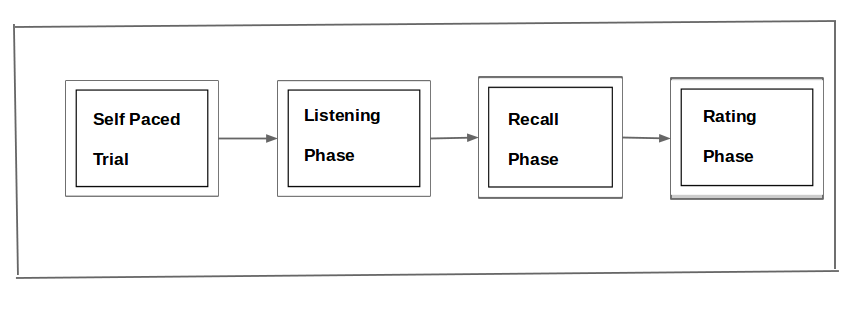
\includegraphics[width=8.5cm]{eval}}
 
%  \vspace{2.0cm}
  \centerline{Fig: Evaluation procedure}\medskip
\end{minipage}
\end{figure}

A set of 15 participants were made to listen to the synthesised equations. Each participant was made to listen to the equations using headphones and the responses were recorded. The listening test was self paced and also the users were informed that they were free to listen to the equation any number of times till they felt comfortable that they could recall the equation.  A similar procedure was followed with equations recorded by trained human speakers. The participant  evaluated the spoken equation based on eight parameters, i.e., perform objective analysis. We arrived at these parameters partly by following the listening test procedures followed in the Blizzard challenges \cite{hinterleitner2011evaluation} and our own analysis.


\subsection{Selection of the equations}
\label{ssec:equations}

Selection  of suitable equations is a critical component to analyse the auditory presentation of mathematical content. We hand picked a few equations which had variations in number of variables, number of sub expressions and length of the equation.  Each of the equations is semantically unrelated. The equations have mathematical content but the listener may not have come across the exact same equation prior to listening to them from our recordings or synthesis. The reason behind choosing such equations is to ensure that the listener's prior knowledge does not influence the ability to recall the equation. This ensures that the user's recall is based on the synthesised equation, not his prior knowledge.

The parameters considered for evaluation include Listening effort (1 = low, 5 = high), Intonation (1 = ineffective and 5 = very effective), Acceptance (1 = poor, 5 = good), Speech pauses ( 1= not noticeable and 5 = very prominent), Accentuation (1 = poor and 5 = very prominent), Content familiarity (1 = totally new concept and 5 = very familiar), Number of repetitions of each equation and Effectiveness of additional cues such as sounds, pitch and rate variations, change in direction, etc. (1 = hardly noticeable and 5 = very helpful). In case of content familiarity, 1 indicates that the user is not acquainted to the terminology used in the equation. The participantÄôs' response for that particular equation can not be considered as he may have entered a wrong response due to the lack of domain knowledge, not due to the lack of understanding of the audio.




\begin{table}[t]
\caption{\label{tts}Evaluation of Spoken Math vs TTS}

\vspace{8pt} % Gap between title and text

% title of Table
\centering
\begin{tabular}{|l |c |c|}
% centered columns (4 columns)
\hline%\hline %inserts double horizontal lines
Parameter & Spoken & Synthesized  \\
                  &              & (Treditional TTS) \\[0.5ex]
% inserts table
%heading
\hline
% inserts single horizontal line

Listening Effort & 2.5 & 4.4 \\
\hline
Content Familiarity &2.7 &2.7 \\
\hline
Effectiveness of & & \\
additional cues &3.2 &1.2 \\
\hline
Accentuation &4.3 &2.5 \\
\hline
Intonation & 4.26 & 1.6  \\
\hline
% inserting body of the table
%Pitch  Variation& 4.17 & 1.4 \\
%\hline
Pauses & 3.1 & 2.15 \\
\hline
Number of repetitions & & \\
(Mode) &2 & 4 \\
\hline
Mean Opinion Score & 4.42 & 1.89  \\%[1ex]
\hline
% [1ex] adds vertical space

%inserts single line


\end{tabular}
\end{table}



\subsection{Inferences from the listening tests}
\label{ssec:basis}
The results of this experiment, shown in the Table ~\ref{tts}   indicate that the equations are not intelligible enough if it is spoken as a plain text using a text-to-speech system. The mean opinion scores of spoken equations indicate a human-being use several acoustic cues to manifest the semantics of the mathematical symbols in audio mode. It was noticed that the trained speakers brought certain variations in their speech while speaking specific aspects of the mathematical expression. The variations are noticed in pauses and pitch variations (intonation). 
A careful analysis revealed that the acoustic variations were introduced by the speakers to unambiguously speak 1) quantification, 2) superscripting and subscripting and 3) fractions in mathematical equations. 

%Sections ~\ref{ssec:quantify} to ~\ref{ssec:fractions}  explain the ambiguities that a listener may come across if the mathematical equation is not spoken with care.

Based on the feedback received from participants, we can infer that the use of these additional cues can effectively and unambiguously present mathematical content in audio.   The question is how to introduce such cues to synthesise a mathematical equation using a text-to-speech system.


\section{Proposed techniques}
\label{sec:techniques}
With the advent of languages like MathML, it is possible to programatically identify different attributes and visual cues of a mathematical expression. This possibility can in turn be leveraged to make some modifications  while generating speech for mathematical content.  We propose four techniques that could enhance the way mathematical content is rendered in audio.


The Equation was first converted into the Math Markup Language format. We chose "Presentation" Markup style to represent the equations.  
It is then text processed to identify and segregate the different terms occurring in the equation. The following terms have been segregated.


The MathML representation is processed to convert it into natural language and the acoustic cues such as pauses, intonation are incorporated to generate a file in the SABLE markup language \cite{sproat1998sable}. 
%Here's an example of the SABLE file:
The SABLE file is input to the speech synthesis system which generates the audio form of the equation with specified pauses and intonation. We have generated the audio files using the Festival Speech Synthesis System\cite{black2002festival}. 
Sections \ref{ssec:t1} through \ref{ssec:t4} discuss each of the four proposed techniques. 



\subsection{ Technique 1 : Rendering equations with pauses and special sounds}
\label{ssec:t1}
 In this concept, we made use of special sounds or ear cons while presenting the equations. However, replacing speech with sounds alone is not the most effective way to tackle the problem of presenting mathematic equations in audio. We made use of additional paralinguistic cues such as  \textbf{Pauses} to convey certain parts of an equation and \textbf{Sounds} to indicate certain symbols and mathematical operations.
Sounds are used to indicate superscripts, subscripts, roots, under scripts, over scripts and under script-over script combination.
We chose the sounds(such as the sound ``ding"Äù) such that would be pleasant to the ear and that are passively noticed by a listener so as not to distract too much, at the same time, are loud enough not to go unnoticed. The sounds show a transition from high to low and low to high when there is a subscript and superscript respectively. Any other type of sounds  and their variations could also be applied in this technique.








\subsection{Technique 2 : Rendering equations with pitch and rate variations}
\label{ssec:t2}

 On observing the human recorded equations explained in Section ~\ref{ssec:basis}, we noticed that speakers tend to modulate the pitch as they read aloud certain parts of a mathematical expression. It has been observed that certain parts of a mathematical expression are spoken at a faster rate to indicate that it is a sub expression and to isolate it from the rest of the expression. \\

In this technique, we use pitch and rate changes to denote the presence of certain mathematical attributes. The pitch and rate increase while speaking out the superscript text and decrease while speaking the subscript text. A similar method is employed to properly render fractions. The numerator is spoken in a higher pitch and the denominator is spoken in a lower pitch. Quantities in a root are spoken at a faster rate. The variation is with respect to the base pitch and rate of the TTS.


\subsection{Technique 3: Rendering equations with audio spatialisation}
\label{ssec:t3}
In this technique, we made an attempt to draw a closer analogy to the spatial positioning of various variables and numbers of a mathematical equation in print. The listener can be given the illusion that the superscript part of the math expression is spoken from above his head and the rest at the usual level using the Head Related Transfer Function (HRTF) \cite{geronazzo2011head}.
Table 
\ref{table:hrtf} shows the sets of angles chosen for the different parts of the equation such as superscript, etc. 



\begin{table}[h]
\caption{Sets of HRTF angles for audio spatialisation}

\vspace{8pt} % Gap between title and tex

% title of Table
\centering
% used for centering table
\begin{tabular}{| c | c | c |}
% centered columns (4 columns)
\hline%\hline %inserts double horizontal lines
Term & Elevation Angle & Azimuth Angle \\[0.5ex]
% inserts table
%heading
\hline
% inserts single horizontal line
Superscript & 90 & 30  \\
% inserting body of the table
Subscript & -90 & 30  \\
Fraction & 270 & 45  \\
Underscript & -90 & 45  \\
Overscript & 90 & 30\\ %[1ex]
% [1ex] adds vertical space
\hline
%inserts single line


\end{tabular}
\label{table:hrtf}
% is used
%to refer this table in the text
\end{table}


We identify the portions of a mathematical expression that require modification in spatial orientation of sound. Based on the attribute, we apply the HRTF function with the required angles.

\begin{table*}[t]
\centering
\caption{Evaluation of the proposed techniques}

\vspace{8pt} % Gap between title and text

% title of Table
%\centering
% used for centering table
\begin{tabularx}{\textwidth}{|l |c |c |c |c|l|}
% centered columns (4 columns)
\hline%\hline %inserts double horizontal lines
Parameter   & Technique\#1 & Technique\#2 & Technique\#3 & Technique\#4 \\[1.5ex]
% inserts table
%heading
\hline
% inserts single horizontal line
Intonation Variation  & 2.3 & \textbf{4.7} & 4.32 & 4.68 \\
\hline
% inserting body of the table
Pitch  Variation & 1.4 & 4.43 & \textbf{4.82} & 4.36\\
\hline
Pauses  & \textbf{4.15} & 3.7 & 3.7 & 3.87 \\
\hline
Listening Effort  & 3.5 & \textbf{2.3} & 2.64 & 2.47\\
\hline
Content Familiarity  &2.7 &2.7 &2.7 &2.7\\
\hline
Effectiveness of additional cues  &1.82 & 4.32 & \textbf{4.37} & 4.23\\
\hline
Accentuation &\textbf{3.47} & 2.3 & 3.2 & 3.6 \\
\hline
Number of repititions(Mode) & 3 & 2 & 2 & 2\\
\hline
Mean Opinion Score  & 2.27 & 4.37 & \textbf{4.62} & 4.35\\ %[1ex]
% [1ex] adds vertical space
\hline
%inserts single line


\end{tabularx}
\label{table:eval}
% is used
%to refer this table in the text
\end{table*}
%\end{center}

  %\centering


\subsection{Technique 4 : Rendering equations with pitch variations and special tones}
\label{ssec:t4}


In this technique, we render the equations in audio by varying the pitch, adding pauses, emphasising the speech and adding sounds at required parts of a mathematical expression. As explained in \ref{ssec:t2} we can make pitch and rate manipulation while rendering superscripts, subscripts, fractions, under scripts and over scripts. In addition to the variations in speech, we have also added sounds to indicate the listener before hand that he must expect one of the above mentioned variations. The sounds used here are the same as the ones mentioned in section \ref{ssec:t1}.
The Pitch and rate variations that are introduced are the same as those used in section \ref{ssec:t2}.


\subsection{Analysis of the Listening test}
\label{ssec:ideaseval}


A system was built to render mathematical expressions implementing each of the proposed ideas. An experiment procedure similar to the one explained in Section \ref{sec:cues} was followed. 30 participants were made to participate in the experiment. The table contains the normalised scores(1 to 5) calculated over the responses for the equations. The number of repetitions of the equation has the  mode value( most occurring value).

On analysing the experiment as described in Section \ref{sec:cues}, it is observed that the participants are able to understand the human spoken equations. More over, it can be clearly understood that generating spoken forms of mathematical equations without making any enhancements is not ideal for rendering math effectively. It can also be inferred that making use of just  a few paralinguistic cues, sounds and pauses as explained in section \ref{ssec:t1} will not suffice either. The pitch and rate changes while rendering certain parts of the mathematical expressions have proven to be helpful to the participants in understanding the expression. In the method described in section \ref{ssec:t3}, the listener has been able to draw an analogy to the print form of mathematics. It has been observed that the method explained in section \ref{ssec:t2} did not prove to be helpful to the listeners. However, from the table \ref{table:eval} and the values corresponding to the technique explained in section \ref{ssec:t4}, it is evident that use of  cues (pauses and rate variations ) in addition to special sounds can be significantly effective in helping a listener.



\section{Evaluating the Comprehension}
\label{sec:comprehension}
 From the evaluation of the techniques presented in table \ref{table:eval}, we could observe that people were able to get a clearer understanding of the equations synthesised using the technique explained in \ref{ssec:t3}. To strengthen this observation further, we performed another experiment to evaluate the comprehendibility of the equations when they are rendered in audio with spatial orientation. We performed this experiment on participants with and without vision loss. The experiment contains equations rendered using a traditional TTS and the idea explained in section \ref{ssec:t3}.The equations contain numbers and basic mathematical operations and are designed such that the participants will be able to solve them mentally. The participant will be made to listen to equations of both  types in random order and he or she will have to enter the response for each of the equations.

\subsection{Evaluation of comprehension test}
\label{ssec:results}

From the table \ref{table:comprehension}, we can observe that participants could solve the equations better when the equations are rendered using the proposed technique. On comparing the results for participants with and without vision impairment, the participants with vision impairment have almost the same correctness rate when compared to those with no vision loss. This observation holds true for equations rendered using our technique(\ref{ssec:t3}). The participants say that the additional verbosity, the pauses and the variations in pitch and rate made understanding the equation an easier task.

\begin{table}[h]
\label{table:comprehension}
\caption{ Accuracy Percentages in Comprehension Evaluation of proposed technique vs TTS}

\vspace{8pt} % Gap between title and text

% title of Table
\centering
\begin{tabular}{|l |c |c|}
% centered columns (4 columns)
\hline%\hline %inserts double horizontal lines
Person & Proposed Technique & Standard TTS  \\
                  &              & (Traditional TTS) \\[0.5ex]
% inserts table
%heading
\hline
% inserts single horizontal line

Normal & 73 & 96 \\
\hline
Visually Challenged & 29.7 & 95 .7 \\
\hline

\hline
% [1ex] adds vertical space

%inserts single line


\end{tabular}
\end{table}



\section{conclusion}
\label{sec:conclusion}

From the analysis and the proposed ideas, we can say that there is a possibility to unambiguously render mathematics in audio. With the increase in voice driven interfaces and information access through audio, rendering mathematical content in audio could also help more effectively present such content in these interfaces. Personal assistance or any other voice driven UIs can more effectively render mathematical content to the listener. In addition to this, effectively rendering mathematical content in audio can be of a great advantage for people with print disabilities including, but not limited to vision  impairment, dyslexia and cognitive impairment. This claim has been validated by the comprehension test. With currently available assistive technology, understanding mathematical content is very difficult and almost impossible. the ideas explained in sections \ref{ssec:t1} to \ref{ssec:t3} improve the scenario  of understanding mathematical content through a non visual input mode. as explained in section \ref{ssec:t4}, There is also a chance that a combination of the proposed ideas are more effective than each of the ideas alone.




% -------------------------------------------------------------------------
\bibliographystyle{IEEEbib}
\bibliography{strings,refs}

\end{document}
